\documentclass[11pt]{amsart}

\usepackage[T1]{fontenc}
\usepackage[utf8]{inputenc}
\usepackage{lmodern}
\usepackage{amsmath,amssymb,amsfonts,amsthm,mathtools,bm,mathrsfs}
\usepackage[a4paper,margin=1in]{geometry}
\usepackage{enumitem,booktabs,array,graphicx,microtype,caption,subcaption}
\usepackage{xcolor,listings,url}
\usepackage[hidelinks]{hyperref}

\numberwithin{equation}{section}
\setcounter{tocdepth}{3}
\setcounter{secnumdepth}{3}

\theoremstyle{plain}
\newtheorem{theorem}{Theorem}[section]
\newtheorem{proposition}[theorem]{Proposition}
\newtheorem{lemma}[theorem]{Lemma}
\newtheorem{corollary}[theorem]{Corollary}
\newtheorem{conjecture}[theorem]{Conjecture}

\theoremstyle{definition}
\newtheorem{definition}[theorem]{Definition}
\newtheorem{experiment}[theorem]{Experiment}

\theoremstyle{remark}
\newtheorem{remark}[theorem]{Remark}

\newcommand{\C}{\mathbb C}
\newcommand{\R}{\mathbb R}
\newcommand{\Hcal}{\mathcal H}
\newcommand{\Pcal}{\mathcal P}
\newcommand{\Ccal}{\mathcal C}
\newcommand{\Ree}{\operatorname{Re}}
\newcommand{\Imm}{\operatorname{Im}}
\newcommand{\Tr}{\operatorname{Tr}}
\newcommand{\dd}{\,\mathrm d}
\newcommand{\ip}[2]{\left\langle #1,#2\right\rangle}
\newcommand{\norm}[1]{\left\lVert #1\right\rVert}
\newcommand{\wedgeHS}{\mathop{\wedge}\limits_{\mathrm{HS}}}

\lstdefinestyle{code}{
  basicstyle=\ttfamily\scriptsize,
  columns=fullflexible,
  breaklines=true,
  breakatwhitespace=false,
  frame=single,
  numbers=left,
  numberstyle=\tiny,
  numbersep=6pt,
  showstringspaces=false,
  keepspaces=true,
  tabsize=4,
  captionpos=b
}
\lstset{style=code}
\captionsetup{font=small}
\setlength{\textfloatsep}{10pt plus 2pt minus 2pt}
\setlength{\floatsep}{8pt plus 2pt minus 2pt}
\renewcommand{\topfraction}{0.92}
\renewcommand{\bottomfraction}{0.85}
\renewcommand{\textfraction}{0.06}
\renewcommand{\floatpagefraction}{0.78}
\raggedbottom

\title[RAINBOW V5]{RAINBOW:\\Violet Thread, Orthogonal-Cubic Projective Geometry, Reflection, P\'olya, and Pluecker Reductions}
\author{Víctor Casaña-Giner}
\address{Bio Logic Crop Science S.L.}
\thanks{ORCID: 0000-0002-8252-2608}
\subjclass[2020]{11M26, 46C05, 15B48, 30B40, 26C10}
\keywords{Rainbow family, Violet fibre, Violet Thread, zero-to-zero lobes, projective Hilbert geometry, orthogonal quotient, total positivity, TP2 kernel, P\'olya frequency sequence, reflection conjugation}
\date{Version 5 --- August 2026}

\begin{document}

\begin{abstract}
For $1/2\le\beta\le1$, the Rainbow family is $W_\beta(t)$, with Violet exactly the fibre $\beta=1/2$.  The primary geometric object is therefore retained at the start of the paper:
\[
W(t)=W_{1/2}(t)=Z(t)e^{-i\vartheta(t)},\qquad
\Gamma(t)=(t,\Re W(t),\Im W(t)).
\]
Its contacts with the value-plane origin are the Violet nodes $\Gamma(\gamma_n)=(\gamma_n,0,0)$, and consecutive nodes delimit the three-dimensional Violet lobes.  Each lobe supplies one fixed phase coordinate $q$, and that coordinate is carried unchanged through the complete Rainbow family; no node is moved or searched as $\beta$ varies.

The orthogonal-cubic quotient $Q_\perp=I-\Pi_3$ produces the projected lobe state $u_{\beta,n}=Q_\perp W_{\beta,n}$ and its projective defect $M_n(\beta)$.  The dense differential audit records $64{,}560/64{,}560$ nonnegative sampled derivatives and $240/240$ complete lobe paths for this quotient, while the corresponding sign law is false for several other fixed quotients.  A separate direct scan of the mixed curvature $\mathcal C(\alpha,\beta)=\partial_{\alpha\beta}\log|K(\alpha,\beta)|$ found no negative sampled values on the reported grids for lobes $2$, $8$, and $25$.

The analytic content is deliberately restricted to unconditional identities, negative results, and explicit open targets.  The Rainbow flow has the fixed generator $L_n=-ia_n(q)\partial_q$.  The projected Gram kernel gives an exact formula for $M'$ and an exact Pluecker representation of the mixed curvature.  The raw modal generator is structurally purely imaginary in every real modal basis, and the constant-coefficient Legendre model admits no fixed diagonal phase gauge making all nonzero couplings cooperative; those routes are closed.  The coherence matrix $R=cc^*$ gives a closed lift of the modal dynamics.  Reflection-conjugation splits the state and the generator into exact symmetric and antisymmetric components and reduces the modal phases to two real sequences.  The Pluecker vector admits both an exact cosine decomposition and an accumulated projective-torsion law.  In parallel, the P\'olya calculation reduces monotone real-negative root flow of the finite modal generating polynomial to the corrected adjacent modal-ratio sign.

No analytic theorem asserting nonvanishing of $u_\beta\wedge u_\beta'$, TP2 on a parameter band, or positivity of $M_n'(\beta)$ on a nontrivial interval is claimed here.  The exact diagonal identity $\mathcal C(\beta,\beta)=P(\beta)\ge0$ holds on the regular projective set, and the remaining global problem is stated directly as the sign of the integrated mixed curvature.  Standard nondegeneracy of the classical Pluecker pairing or Grassmannian does not settle the possible vanishing of the specific Rainbow bivector $u_\beta\wedge u_\beta'$ and is not used as a substitute.
\end{abstract}

\maketitle
\tableofcontents
\bigskip

\section{Rainbow and the Violet fibre}
\label{sec:rainbow}

\begin{definition}[Rainbow family and Violet fibre]
\label{def:rainbow}
For
\begin{equation}
\frac12\le\beta\le1,
\label{eq:beta-domain}
\end{equation}
define the Rainbow functions
\begin{equation}
\boxed{
W_\beta(t)=\zeta(\beta+it).
}
\label{eq:Rainbow-functions}
\end{equation}
The complete family $\{W_\beta\}_{1/2\le\beta\le1}$ is called \emph{Rainbow}.  Its distinguished fibre
\begin{equation}
\boxed{
W(t):=W_{1/2}(t)=\zeta\!\left(\frac12+it\right)=u(t)+iv(t)
}
\label{eq:W-definition}
\end{equation}
is called \emph{Violet}.
\end{definition}

The central three-dimensional Violet trace is
\begin{equation}
\boxed{
\Gamma(t)=\bigl(t,u(t),v(t)\bigr).
}
\label{eq:Gamma-definition}
\end{equation}
The classical Hardy decomposition \cite{Titchmarsh1986} is
\begin{equation}
\boxed{
W(t)=Z(t)e^{-i\vartheta(t)},
\qquad Z(t)\in\R.
}
\label{eq:Hardy-decomposition}
\end{equation}
Consequently
\begin{equation}
\Gamma(t)=\bigl(t,Z(t)\cos\vartheta(t),-Z(t)\sin\vartheta(t)\bigr).
\label{eq:cylindrical-thread}
\end{equation}
Differentiation gives
\begin{equation}
W_t(t)=e^{-i\vartheta(t)}\bigl(Z'(t)-i\vartheta'(t)Z(t)\bigr)
\label{eq:Wt-Hardy}
\end{equation}
and hence
\begin{equation}
|W_t(t)|^2=Z'(t)^2+\vartheta'(t)^2Z(t)^2.
\label{eq:speed-Hardy}
\end{equation}

\begin{figure}[tbp]
\centering
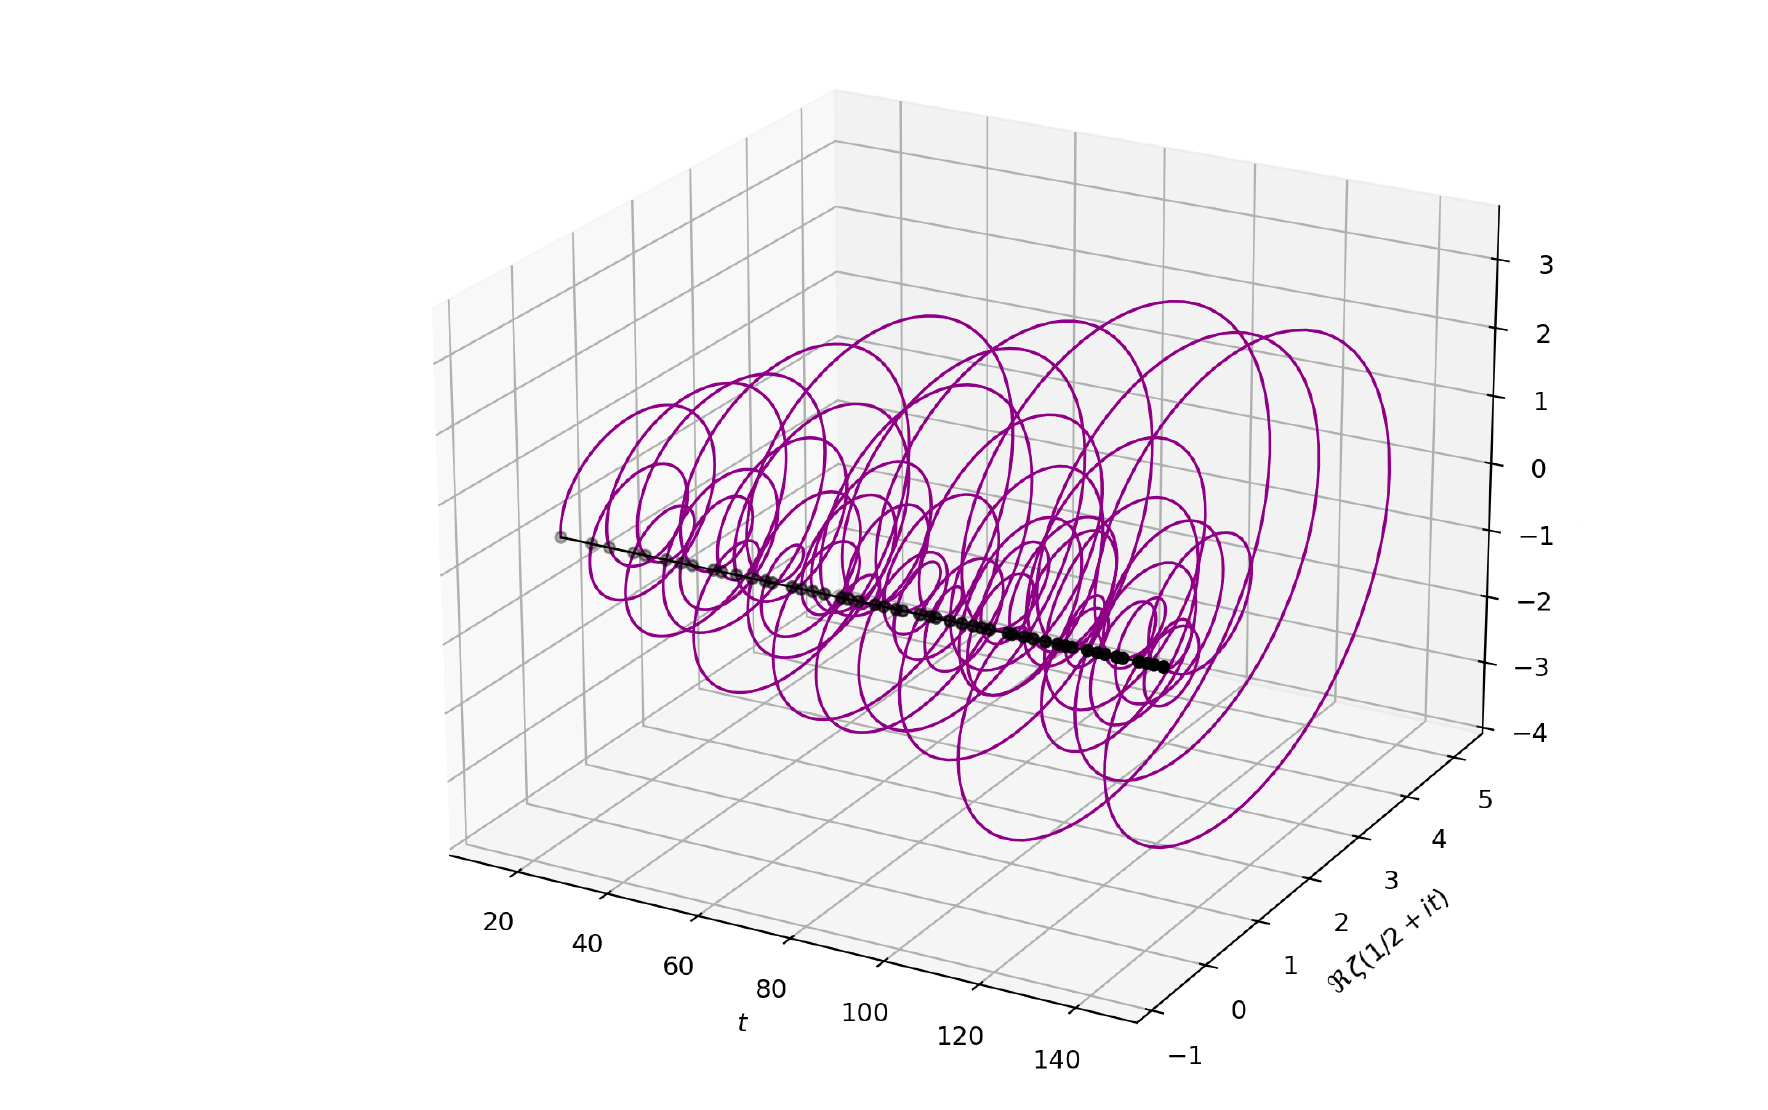
\includegraphics[width=.82\textwidth]{../figures/fig01_euclidean_violet_thread.png}
\caption{The Euclidean Violet Thread over the first fifty carried node ordinates.  The black points are the contacts $\Gamma(\gamma_n)=(\gamma_n,0,0)$; each violet arc between consecutive contacts is one genuine three-dimensional lobe.}
\label{fig:violet-thread}
\end{figure}

\subsection{Violet nodes and zero-to-zero lobes}
\label{subsec:nodes-lobes}

Let $\gamma_n<\gamma_{n+1}$ be consecutive contacts of the Violet trace with the value-plane origin:
\begin{equation}
\boxed{
W(\gamma_n)=0,
\qquad
\Gamma(\gamma_n)=(\gamma_n,0,0).
}
\label{eq:Violet-nodes}
\end{equation}
The $n$th Violet lobe is the curve segment
\begin{equation}
\boxed{
\mathcal L_n
=
\left\{\Gamma(t):\gamma_n\le t\le\gamma_{n+1}\right\}.
}
\label{eq:Violet-lobe}
\end{equation}
On
\begin{equation}
I_n=(\gamma_n,\gamma_{n+1})
\label{eq:lobe-interval}
\end{equation}
the sign of $Z$ is constant.  Put
\begin{equation}
\varepsilon_n=\operatorname{sgn}Z(t),
\qquad t\in I_n,
\label{eq:epsilon-n}
\end{equation}
and define the fixed phase sweep
\begin{equation}
\Omega_n=\vartheta(\gamma_{n+1})-\vartheta(\gamma_n).
\label{eq:Omega}
\end{equation}
Rotate only by the fixed Violet lobe phase:
\begin{equation}
\widehat W_{V,n}(t)
=\varepsilon_n e^{i\vartheta(\gamma_n)}W(t)
=|Z(t)|e^{-i[\vartheta(t)-\vartheta(\gamma_n)]}.
\label{eq:rotated-Violet-lobe}
\end{equation}

Introduce the uniform lobe phase coordinate
\begin{equation}
q=\frac{\vartheta(t)-\vartheta(\gamma_n)}{\Omega_n},
\qquad 0\le q\le1,
\label{eq:q-phase}
\end{equation}
or equivalently define $t_n(q)$ by
\begin{equation}
\boxed{
\vartheta(t_n(q))=\vartheta(\gamma_n)+\Omega_n q.
}
\label{eq:tq}
\end{equation}
With
\begin{equation}
r_n(q)=|Z(t_n(q))|,
\label{eq:rn}
\end{equation}
the rotated Violet lobe is exactly
\begin{equation}
\boxed{
\widehat W_{V,n}(q)=r_n(q)e^{-i\Omega_n q},
\qquad
r_n(0)=r_n(1)=0.
}
\label{eq:Violet-lobe-polar}
\end{equation}
Thus the node--lobe--node geometry is retained before any quotient or projective construction is introduced.

\begin{figure}[tbp]
\centering
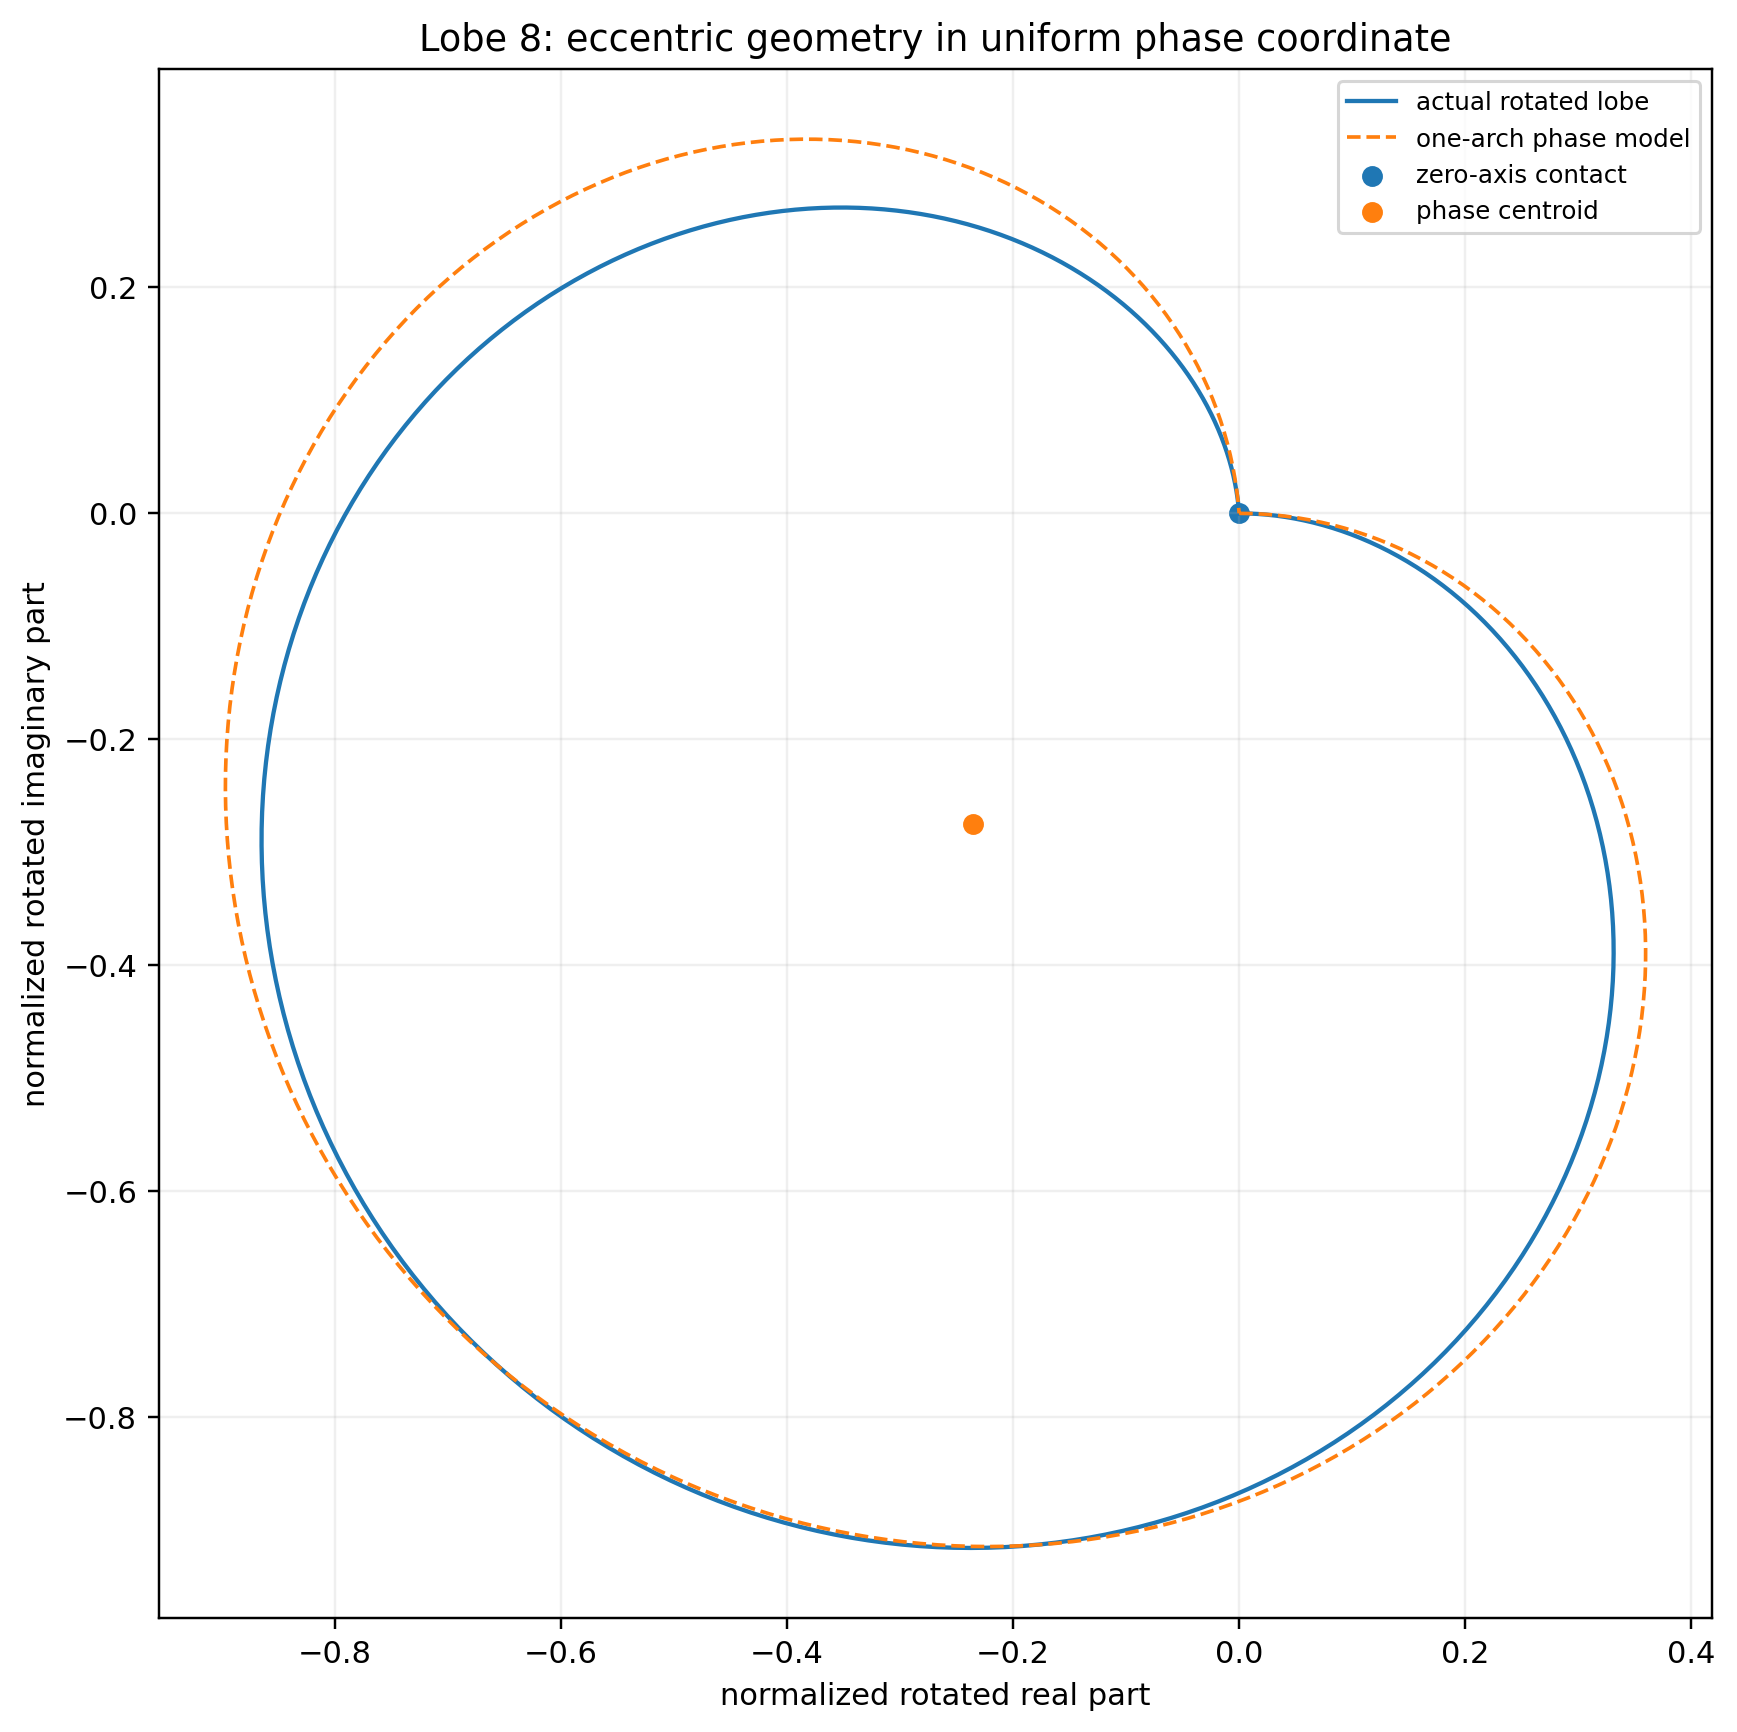
\includegraphics[width=.68\textwidth]{../figures/fig02_single_lobe_phase_geometry.png}
\caption{A representative Violet lobe in the uniform phase coordinate.  The two endpoints are the consecutive Violet nodes; the fixed map $q\mapsto t_n(q)$ is the coordinate carried into every Rainbow fibre.}
\label{fig:single-lobe-phase}
\end{figure}

\subsection{Rainbow lobe fibres}
\label{subsec:rainbow-lobes}

The Rainbow deformation does not move the Violet nodes.  Instead, each Violet interval and its phase coordinate are frozen and used to sample every fibre:
\begin{equation}
\boxed{
W_{\beta,n}(q)=W_\beta(t_n(q)),
\qquad
\frac12\le\beta\le1.
}
\label{eq:Rainbow-lobe-fibre}
\end{equation}
At $\beta=1/2$ this is exactly the original Violet lobe before the fixed phase rotation.  For $\beta>1/2$, the values at $q=0,1$ are not declared to be nodes; the endpoints remain the fixed Violet coordinates $\gamma_n,\gamma_{n+1}$.

The same fixed rotation may be applied throughout the family,
\begin{equation}
\widehat W_{\beta,n}(q)
=\varepsilon_n e^{i\vartheta(\gamma_n)}W_{\beta,n}(q),
\label{eq:rotated-Rainbow-lobe}
\end{equation}
and is projectively immaterial because the multiplier is independent of $\beta$ and $q$.  In the remainder of the paper $W_{\beta,n}$ denotes the unrotated Rainbow fibre unless a rotated lobe is explicitly required.

\section{Fixed Rainbow transverse generator}
\label{sec:generator}

Put
\begin{equation}
F(\delta,t)=W_{1/2+\delta}(t),
\qquad \delta=\beta-\frac12.
\label{eq:F-delta}
\end{equation}
Analyticity gives the exact quarter-turn identity
\begin{equation}
\boxed{F_\delta=-iF_t.}
\label{eq:quarter-turn}
\end{equation}
Differentiating \eqref{eq:tq} yields
\begin{equation}
\vartheta'(t_n(q))t_n'(q)=\Omega_n.
\label{eq:tq-derivative}
\end{equation}
Hence every fixed Violet lobe generates the autonomous Rainbow evolution
\begin{equation}
\boxed{
\partial_\beta W_{\beta,n}
=L_nW_{\beta,n},
\qquad
L_n=-ia_n(q)\partial_q,
\qquad
a_n(q)=\frac{\vartheta'(t_n(q))}{\Omega_n}.
}
\label{eq:fixed-generator}
\end{equation}
The coefficient $a_n$ depends on the fixed Violet lobe coordinate but not on $\beta$.

\begin{proposition}[Fixed-generator Rainbow evolution]
\label{prop:fixed-generator}
For each fixed lobe, \eqref{eq:fixed-generator} is an autonomous evolution in the Rainbow parameter $\beta$.  On analytic vectors it is equivalent to the exact complex translation generated by $-i\partial_t$.
\end{proposition}

\begin{proof}
Equation~\eqref{eq:quarter-turn} is $\partial_\delta F=(-i\partial_t)F$.  Since $t_n(q)$ is fixed once the Violet lobe is chosen, the chain rule converts $-i\partial_t$ to $-ia_n(q)\partial_q$, with no residual $\beta$ dependence.
\end{proof}

\begin{figure}[tbp]
\centering
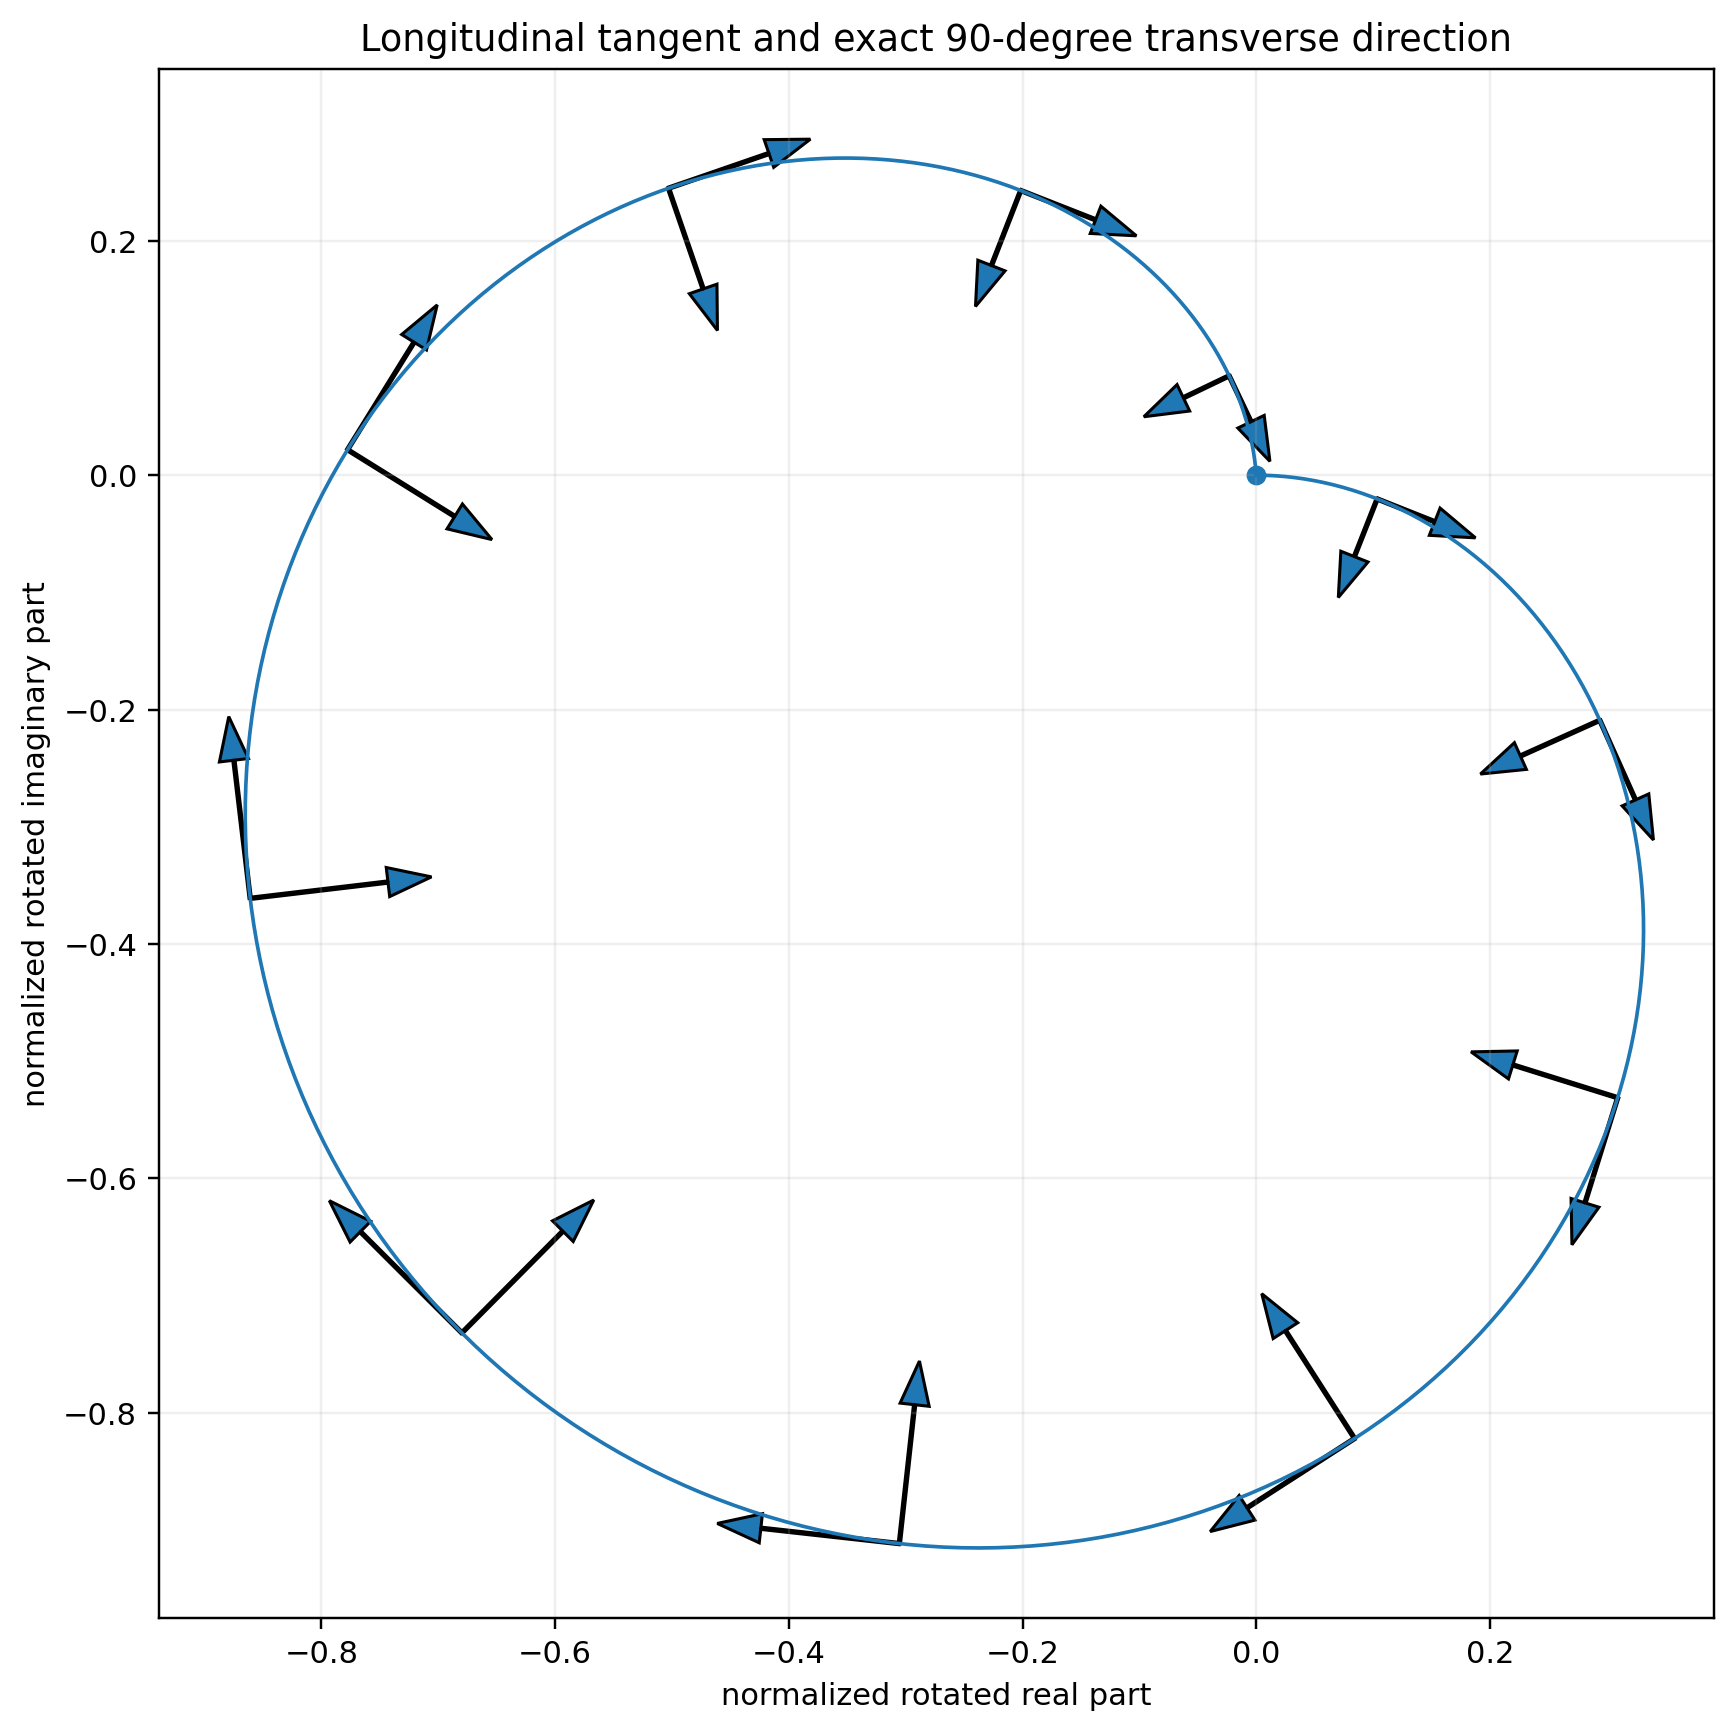
\includegraphics[width=.70\textwidth]{../figures/fig03_quarter_turn_vector_field.png}
\caption{Exact transverse quarter-turn field on a Violet lobe.  This is the geometric origin of the fixed Rainbow generator $L_n=-ia_n(q)\partial_q$.}
\label{fig:quarter-turn}
\end{figure}

\begin{lemma}[Internal variation of the Rainbow coefficient]
\label{lem:a-prime}
One has the exact identity
\begin{equation}
\boxed{
a_n'(q)=\frac{\vartheta''(t_n(q))}{\vartheta'(t_n(q))}.
}
\label{eq:a-prime}
\end{equation}
\end{lemma}

\begin{proof}
Differentiate $a_n(q)=\vartheta'(t_n(q))/\Omega_n$ and use $t_n'(q)=\Omega_n/\vartheta'(t_n(q))$.
\end{proof}

\section{Scope and logical status}
\label{sec:scope}

The primary objects of this paper are the Rainbow family $W_\beta$, its Violet fibre $W=W_{1/2}$, the Violet nodes $\gamma_n$, the Violet lobes $\mathcal L_n$, and the fixed lobe flow \eqref{eq:fixed-generator}.  The formula \eqref{eq:Rainbow-functions} defines the family; after that definition, the proof program developed below is internal to these Rainbow objects: fixed lobe coordinates, orthogonal projection, projective geometry, modal transport, reflection, coherence matrices, P\'olya root flow, and Pluecker bivectors.

No function $\gamma_n(\beta)$ is introduced.  No node is transported or searched away from Violet.  Numerical evaluators are used only to evaluate the already defined Rainbow fibres in the finite experiments.  Exact identities, finite computations, negative results, and unresolved analytic targets are kept distinct throughout.

\section{The orthogonal-cubic quotient}
\label{sec:quotient}

Let
\begin{equation}
\Hcal=L^2([0,1],\dd q;\C),
\qquad
\ip{f}{g}=\int_0^1\overline{f(q)}g(q)\dd q.
\end{equation}
Define
\begin{equation}
\Pcal_3=\operatorname{span}\{1,q,q^2,q^3\},
\qquad
Q_\perp=I-\Pi_3,
\label{eq:Qperp}
\end{equation}
where $\Pi_3$ is the orthogonal projection onto $\Pcal_3$.  Set
\begin{equation}
u_{\beta,n}=Q_\perp W_{\beta,n},
\qquad
r_{\beta,n}=\frac{u_{\beta,n}}{\norm{u_{\beta,n}}}.
\label{eq:u-r}
\end{equation}
For $\beta_0=1/2$ define the projective defect
\begin{equation}
\boxed{
M_n(\beta)=1-\left|\ip{r_{\beta_0,n}}{r_{\beta,n}}\right|^2.
}
\label{eq:M}
\end{equation}

\begin{proposition}[Canonical quotient metric]
\label{prop:quotient}
$Q_\perp f$ is the unique minimum-norm representative of the quotient class $[f]\in\Hcal/\Pcal_3$, and
\begin{equation}
\ip{[f]}{[g]}_{\Hcal/\Pcal_3}
:=\ip{Q_\perp f}{Q_\perp g}
\end{equation}
defines the natural Hilbert inner product on the quotient.
\end{proposition}

\begin{proof}
The orthogonal decomposition $f=\Pi_3f+Q_\perp f$ gives
\begin{equation}
\norm{Q_\perp f+p}^2=\norm{Q_\perp f}^2+\norm{p}^2
\end{equation}
for $p\in\Pcal_3$.  The minimum and representative-independence follow immediately.
\end{proof}

\section{Finite quotient and differential audits}
\label{sec:numerics}

The quotient-rigidity computation used $240$ consecutive lobes, a $49$-point $\beta$ grid, and five fixed linear quotients.  Four gave $240/240$ discretely monotone lobe paths; the endpoint-only quotient gave $235/240$.  The intersection across all five quotients was $235/240$.  This establishes robustness of the ordering at the sampled scale, but not a differential law.

\begin{figure}[t]
\centering
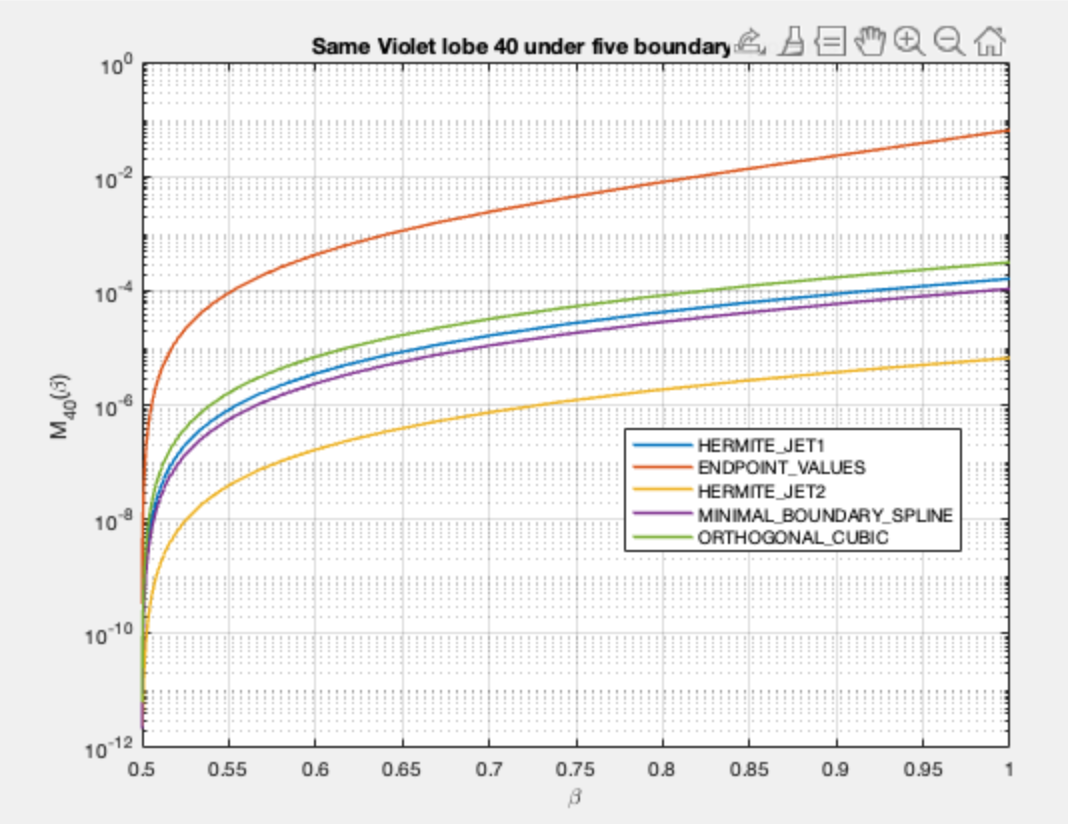
\includegraphics[width=.82\textwidth,trim=0 0 0 45,clip]{../figures/fig04_quotient_rigidity_lobe40.png}
\caption{Projective defect of lobe $40$ under five fixed quotient constructions.  The top application chrome and plot title are clipped; the plotted data are unchanged.  The quotient changes the scale substantially while preserving the sampled ordering for this lobe.}
\label{fig:quotient-lobe40}
\end{figure}

The denser differential audit used $270$ $\beta$ samples.  The universal cross-quotient statement is false.  The orthogonal-cubic quotient, however, was the only tested quotient with no sampled differential failure.

\begin{table}[t]
\centering
\caption{Dense differential audit on $240$ lobes.}
\label{tab:differential}
\begin{tabular}{lrrr}
\toprule
Quotient & Nonnegative samples & Lobes all-beta & Minimum $M'_{n}$\\
\midrule
Hermite jet 1 & $64556/64560$ & $239/240$ & $-4.063\times10^{-9}$\\
Endpoint values & $64299/64560$ & $227/240$ & $-8.741$\\
Hermite jet 2 & $62735/64560$ & $182/240$ & $-9.120\times10^{-7}$\\
Minimal boundary spline & $64544/64560$ & $239/240$ & $-1.179\times10^{-7}$\\
Orthogonal cubic & $64560/64560$ & $240/240$ & $+3.412\times10^{-10}$\\
\bottomrule
\end{tabular}
\end{table}

\begin{figure}[t]
\centering
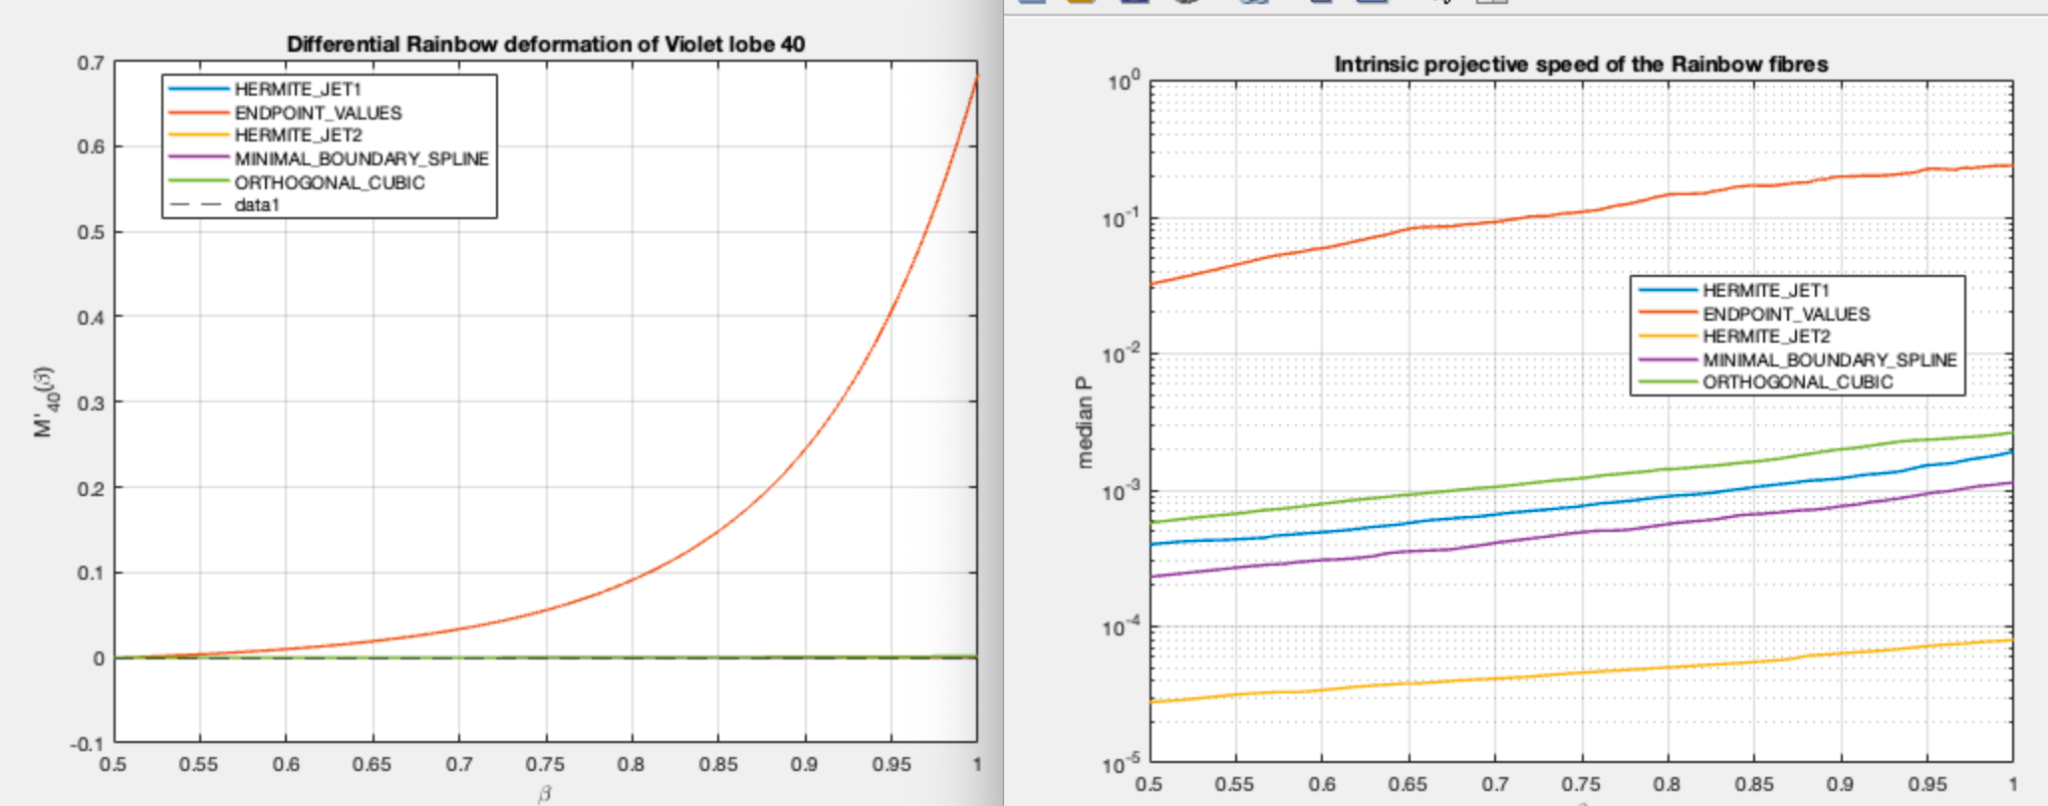
\includegraphics[width=.98\textwidth,trim=0 0 0 82,clip]{../figures/fig05_projective_flow.png}
\caption{Differential lobe-$40$ deformation and median intrinsic projective speed from the dense audit.  The original panel titles are clipped; no data are altered.}
\label{fig:differential-flow}
\end{figure}

The orthogonal-cubic row motivates the sign problem
\begin{equation}
\boxed{
M_n'(\beta)\stackrel{?}{\ge}0,
\qquad \frac12\le\beta\le1.
}
\label{eq:main-conjecture}
\end{equation}
The finite audit does not prove \eqref{eq:main-conjecture}.

\section{Projected Gram kernel and exact mixed curvature}
\label{sec:kernel}

For the rest of the analytic discussion, $Q=Q_\perp$ and the lobe index is suppressed.  Define
\begin{equation}
K(\alpha,\beta)=\ip{u_\alpha}{u_\beta}.
\label{eq:K}
\end{equation}
Then
\begin{equation}
1-M(\beta)=\frac{|K(\beta_0,\beta)|^2}{K(\beta_0,\beta_0)K(\beta,\beta)}.
\label{eq:M-K}
\end{equation}
On any connected region where $K\ne0$, define
\begin{equation}
\Ccal(\alpha,\beta)=\partial_\alpha\partial_\beta\log|K(\alpha,\beta)|.
\label{eq:C}
\end{equation}

\begin{theorem}[Exact projective derivative]
\label{thm:Mprime}
One has
\begin{equation}
\boxed{
M'(\beta)=2(1-M(\beta))
\int_{\beta_0}^{\beta}\Ccal(\alpha,\beta)\dd\alpha.
}
\label{eq:Mprime-C}
\end{equation}
Moreover
\begin{equation}
\Ccal(\alpha,\beta)
=\Ree\left[
\frac{\ip{u_\alpha'}{u_\beta'}}{K(\alpha,\beta)}
-\frac{\ip{u_\alpha'}{u_\beta}\ip{u_\alpha}{u_\beta'}}{K(\alpha,\beta)^2}
\right].
\label{eq:C-explicit}
\end{equation}
\end{theorem}

\begin{proof}
Taking logarithms of \eqref{eq:M-K} and differentiating gives
\begin{equation}
M'(\beta)=2(1-M)
\left[
\partial_\beta\log|K(\beta,\beta)|^{1/2}
-\partial_\beta\log|K(\beta_0,\beta)|
\right].
\end{equation}
The fundamental theorem of calculus in the first kernel variable gives \eqref{eq:Mprime-C}.  Differentiating $\log|K|$ in both variables gives \eqref{eq:C-explicit}.
\end{proof}

Define the intrinsic projective speed
\begin{equation}
P(\beta)
=\frac{\norm{u_\beta'}^2}{\norm{u_\beta}^2}
-\frac{|\ip{u_\beta}{u_\beta'}|^2}{\norm{u_\beta}^4}.
\label{eq:P}
\end{equation}

\begin{proposition}[Exact diagonal projective identity]
\label{prop:diagonal}
On the regular projective set $u_\beta\ne0$,
\begin{equation}
\boxed{\Ccal(\beta,\beta)=P(\beta)\ge0.}
\label{eq:Cdiag}
\end{equation}
Equivalently,
\begin{equation}
\boxed{
\Ccal(\beta,\beta)
=\frac{\norm{u_\beta\wedge u_\beta'}^2}{\norm{u_\beta}^4}.
}
\label{eq:Cdiag-wedge}
\end{equation}
\end{proposition}

\begin{proof}
Set $\alpha=\beta$ in \eqref{eq:C-explicit} and use the Hilbert-space Lagrange identity
\begin{equation}
\norm{u\wedge v}^2=\norm{u}^2\norm{v}^2-|\ip{u}{v}|^2.
\end{equation}
\end{proof}

The stronger pointwise target is
\begin{equation}
\boxed{
\Ccal(\alpha,\beta)\ge0,
\qquad \beta_0\le\alpha\le\beta\le1.
}
\label{eq:TP2-target}
\end{equation}
For $|K|>0$, this is the differential TP2/log-supermodularity condition for $|K|$.  It is stronger than the integrated condition actually equivalent to $M'\ge0$.

\section{Supplementary direct pointwise-curvature scan}
\label{sec:Cscan}

The preceding differential experiment tested $M'$ directly.  A later direct calculation evaluated \eqref{eq:C-explicit} itself for the orthogonal-cubic quotient using the same Rainbow fibre evaluator.  The supplied development log records the following interior-pair results.

\begin{table}[t]
\centering
\caption{Direct pointwise mixed-curvature scan for the orthogonal-cubic quotient.  Endpoints are omitted from the displayed pair counts.}
\label{tab:Cscan}
\begin{tabular}{rrrrr}
\toprule
Lobe & $\beta$ grid & Interior pairs & $\min\Ccal$ & $\max\Ccal$\\
\midrule
2  & 11 points & 81  & $9.0\times10^{-5}$ & $1.1\times10^{-4}$\\
8  & 21 points & 361 & $1.64\times10^{-3}$ & $2.49\times10^{-3}$\\
25 & 11 points & 81  & $8.8\times10^{-4}$ & $1.50\times10^{-3}$\\
\bottomrule
\end{tabular}
\end{table}

No negative value was reported in any of the $523$ displayed interior pairs.  This is stronger finite evidence than the direct $M'$ scan because it targets the stronger pointwise condition \eqref{eq:TP2-target}.  It remains a finite computation.  Appendix~\ref{app:matlab-reflection} contains a MATLAB reconstruction of the pointwise-curvature calculation together with the later reflection and modal diagnostics.

\section{Diagonal curvature and exact far-memory decomposition}
\label{sec:far-memory}

The diagonal identity \eqref{eq:Cdiag} is exact, but it does not by itself give an off-diagonal sign.  Version~5 therefore makes no analytic TP2-band claim.  The direct scan in Table~\ref{tab:Cscan} is retained as finite evidence only.

The projective integral can nevertheless be separated exactly at any chosen radius $r>0$.  For $\beta-r\ge\beta_0=1/2$, define, on a connected region where the displayed kernel logarithms are regular,
\begin{equation}
I_{\mathrm{near}}^{(r)}(\beta)
=\int_{\beta-r}^{\beta}\Ccal(\alpha,\beta)\dd\alpha,
\label{eq:Inear}
\end{equation}
\begin{equation}
I_{\mathrm{far}}^{(r)}(\beta)
=\int_{\beta_0}^{\beta-r}\Ccal(\alpha,\beta)\dd\alpha.
\label{eq:Ifar}
\end{equation}
Then
\begin{equation}
\boxed{
\frac{M'(\beta)}{2(1-M(\beta))}
=I_{\mathrm{far}}^{(r)}(\beta)+I_{\mathrm{near}}^{(r)}(\beta).
}
\label{eq:Ifar-Inear}
\end{equation}
No sign is assigned analytically to either term in Version~5.

Put
\begin{equation}
g(\alpha,\beta)=\partial_\beta\log|K(\alpha,\beta)|.
\label{eq:g-kernel}
\end{equation}
Since $\Ccal=\partial_\alpha g$, the far contribution collapses exactly to two boundary rates:
\begin{equation}
\boxed{
I_{\mathrm{far}}^{(r)}(\beta)
=g(\beta-r,\beta)-g(\beta_0,\beta).
}
\label{eq:far-memory-boundary}
\end{equation}
Thus the global problem does not require pointwise positivity on the whole parameter triangle.  It requires control of the total integral in \eqref{eq:Mprime-C}; \eqref{eq:far-memory-boundary} isolates the genuinely nonlocal part without assuming any positive near-diagonal margin.

The first transverse derivative of the mixed curvature is also explicit wherever $K\ne0$:
\begin{equation}
\boxed{
\partial_\alpha\Ccal
=\Ree\left[
\frac{K_{\alpha\alpha\beta}}{K}
-\frac{2K_\alpha K_{\alpha\beta}+K_{\alpha\alpha}K_\beta}{K^2}
+\frac{2K_\alpha^2K_\beta}{K^3}
\right].
}
\label{eq:C-alpha-derivative}
\end{equation}
This formula is recorded as a quantitative tool.  No bound extracted from it is promoted to a positivity theorem without an independent Rainbow proof of the missing nonvanishing and lower-margin information.

\section{Why the naive cooperative-generator route fails}
\label{sec:no-go}

The fixed generator is structurally constrained.  Let $\{\phi_m\}$ be any real orthonormal basis.  Since $a_n(q)$ and $\phi_m$ are real,
\begin{equation}
G_{mk}^{(n)}
:=\ip{\phi_m}{L_n\phi_k}
=-iD_{mk}^{(n)},
\qquad
D_{mk}^{(n)}\in\R.
\label{eq:Gimag}
\end{equation}
Thus the modal matrix is purely imaginary for every lobe.  If $c=x+iy$, then
\begin{equation}
\dot x=D y,
\qquad
\dot y=-D x
\end{equation}
up to the chosen sign convention for $D$.  The dynamics are cross-coupled and cannot be read as a real Metzler system in either $x$ or $y$ separately.

There is a stronger obstruction even in the constant-coefficient model.

\begin{proposition}[No fixed cooperative phase gauge in the Legendre transport model]
\label{prop:no-gauge}
Let
\begin{equation}
\phi_m(q)=\sqrt{2m+1}\,P_m(2q-1)
\end{equation}
be the normalized shifted Legendre basis and suppose $a(q)\equiv a_0>0$.  There is no fixed diagonal phase gauge $a_m=e^{i\omega_m}b_m$ that makes every nonzero off-diagonal entry of the modal generator real and positive.
\end{proposition}

\begin{proof}
The exact derivative identity is
\begin{equation}
\phi_k'(q)
=2\sum_{\substack{m<k\\k-m\;\mathrm{odd}}}
\sqrt{(2m+1)(2k+1)}\,\phi_m(q).
\label{eq:legendre-derivative}
\end{equation}
Hence the entries $G_{4,5}$, $G_{5,6}$, $G_{6,7}$, and $G_{4,7}$ are all nonzero and have phase $-\pi/2$.  Positivity after the diagonal phase gauge would require
\begin{equation}
\omega_5-\omega_4\equiv\omega_6-\omega_5\equiv\omega_7-\omega_6\equiv\frac\pi2\pmod{2\pi}.
\end{equation}
The first three relations imply $\omega_7-\omega_4\equiv3\pi/2$, whereas the direct $4\to7$ coupling requires $\omega_7-\omega_4\equiv\pi/2$.  Contradiction.
\end{proof}

Therefore a proof of \eqref{eq:main-conjecture} cannot follow solely from a hidden Metzler structure of $Q_\perp L_nQ_\perp$.

\subsection{Formal self-adjoint/rotational split}

Boundary terms aside, the formal adjoint is
\begin{equation}
L_n^*=L_n-ia_n'(q).
\end{equation}
Write
\begin{equation}
L_n=A_n+iB_n,
\end{equation}
with
\begin{equation}
\boxed{
A_n=-i\sqrt{a_n}\,\partial_q\sqrt{a_n},
\qquad
B_n=\frac12a_n'(q).
}
\label{eq:AB}
\end{equation}
These are formally self-adjoint under compatible domain conditions.  Their noncommutation is explicit:
\begin{equation}
\boxed{
[A_n,B_n]=-\frac{i}{2}a_n(q)a_n''(q)
}
\label{eq:commutator}
\end{equation}
as a multiplication operator.  Thus the relevant commutator is governed by $a_na_n''$, not merely by the size of $a_n'$.

\section{Modal equations and the corrected Chebyshev sign}
\label{sec:modal}

Use the real shifted-Legendre basis and expand the full state
\begin{equation}
W_\beta=\sum_{m\ge0}c_m(\beta)\phi_m.
\end{equation}
Because the full generator is autonomous,
\begin{equation}
\boxed{c'=-iDc,}
\label{eq:c-full}
\end{equation}
where $D$ is a real matrix.  Splitting low and high modes,
\begin{equation}
c=(c_L,c_H),
\qquad
c_H=(c_4,c_5,\ldots),
\end{equation}
recovers the projected equation
\begin{equation}
c_H'=-iD_{HH}c_H-iD_{HL}c_L.
\label{eq:high-forced}
\end{equation}
The second term is exactly the modal form of $Q_\perp L\Pi_3W$; it is not an independent source.

Let
\begin{equation}
p_m=|c_m|^2.
\end{equation}
Then
\begin{equation}
\boxed{
p_m'
=2\sum_kD_{mk}\Imm(\overline{c_m}c_k).
}
\label{eq:pprime}
\end{equation}
Consequently the $p_m$ do not form a closed system; the relative modal phases enter through the coherences $\Imm(\overline{c_m}c_k)$.

For adjacent high modes define
\begin{equation}
\boxed{
\Delta_m(\beta)
=p_m p_{m+1}'-p_{m+1}p_m'.
}
\label{eq:Delta-correct}
\end{equation}
This sign is the corrected one.  Wherever $p_mp_{m+1}>0$,
\begin{equation}
\boxed{
\Delta_m\ge0
\iff
\frac{\dd}{\dd\beta}\log\frac{p_{m+1}}{p_m}\ge0
\iff
\frac{\dd}{\dd\beta}\log\frac{|c_{m+1}|}{|c_m|}\ge0.
}
\label{eq:RC}
\end{equation}
The previously reversed $2\times2$ determinant sign is not used in this version.

\section{The coherence matrix: a closed lift of the modal dynamics}
\label{sec:coherence}

The correct closed object one level above $p_m$ is
\begin{equation}
\boxed{R(\beta)=c(\beta)c(\beta)^*.}
\label{eq:R}
\end{equation}
From \eqref{eq:c-full},
\begin{equation}
\boxed{
R'=-iDR+iRD^T.
}
\label{eq:Rflow}
\end{equation}
This equation contains the modal moduli and all phase coherences simultaneously.

Let $P$ denote the diagonal projection onto indices $m\ge4$ and set
\begin{equation}
\widehat R_\beta=PR_\beta P.
\end{equation}
Then
\begin{equation}
\boxed{
|K(\alpha,\beta)|^2
=\Tr(\widehat R_\alpha\widehat R_\beta).
}
\label{eq:K-R}
\end{equation}
Thus the squared absolute kernel is itself a Gram kernel in the real Hilbert space of Hermitian Hilbert--Schmidt operators.

For
\begin{equation}
S(\alpha,\beta)=|K(\alpha,\beta)|^2,
\end{equation}
TP2 of $|K|$ is equivalent to TP2 of $S$, because $S=|K|^2$ and all entries are nonnegative.  The $2\times2$ minor has the exterior-algebra representation
\begin{equation}
\boxed{
\det\bigl(S(\alpha_i,\beta_j)\bigr)_{i,j=1}^2
=
\ip{
\widehat R_{\alpha_1}\wedgeHS\widehat R_{\alpha_2}
}{
\widehat R_{\beta_1}\wedgeHS\widehat R_{\beta_2}
}_{\wedge^2\mathrm{HS}}.
}
\label{eq:HS-wedge}
\end{equation}
Hence the phase problem can be phrased as a cone problem for ordered Hilbert--Schmidt bivectors rather than as a demand for exact locking of every individual phase.

\section{Reflection-conjugation reduction}
\label{sec:reflection}

Let $\mathcal R$ denote reflection, $(\mathcal R f)(q)=f(1-q)$.  For a fixed real parameter $\chi$ define
\begin{equation}
\boxed{
(J_\chi f)(q)=e^{2i\chi}\overline{f(1-q)}.
}
\label{eq:J}
\end{equation}
$J_\chi$ is an antiunitary involution.  Since $\Pcal_3$ is real and invariant under $q\mapsto1-q$,
\begin{equation}
\boxed{J_\chi Q_\perp=Q_\perp J_\chi.}
\label{eq:JQ}
\end{equation}

Split
\begin{equation}
a_+(q)=\frac{a(q)+a(1-q)}2,
\qquad
a_-(q)=\frac{a(q)-a(1-q)}2,
\end{equation}
and
\begin{equation}
L_\pm=-ia_\pm(q)\partial_q.
\end{equation}

\begin{lemma}[Exact reflection parity of the generator]
\label{lem:JL}
\begin{equation}
\boxed{
J_\chi L_+J_\chi=L_+,
\qquad
J_\chi L_-J_\chi=-L_-.
}
\label{eq:JL}
\end{equation}
\end{lemma}

\begin{proof}
For $L_a=-ia(q)\partial_q$, direct differentiation gives
\begin{equation}
J_\chi L_aJ_\chi=-ia(1-q)\partial_q.
\end{equation}
Apply this to the symmetric and antisymmetric parts of $a$.
\end{proof}

Define
\begin{equation}
X_\beta=\frac{W_\beta+J_\chi W_\beta}{2},
\qquad
Y_\beta=\frac{W_\beta-J_\chi W_\beta}{2}.
\label{eq:XY}
\end{equation}
Then $J_\chi X=X$ and $J_\chi Y=-Y$.

\begin{proposition}[Exact coupled reflection system]
\label{prop:XYflow}
The transverse evolution is equivalent to
\begin{equation}
\boxed{
\begin{aligned}
X_\beta'&=L_+X_\beta+L_-Y_\beta,\\
Y_\beta'&=L_+Y_\beta+L_-X_\beta.
\end{aligned}}
\label{eq:XYflow}
\end{equation}
Thus departure from the $J_\chi$-fixed subspace has exactly two sources: the initial defect $Y_{\beta_0}$ and the antisymmetric forcing $L_-X$.
\end{proposition}

\begin{proof}
Use $W=X+Y$, $J_\chi W=X-Y$, and \eqref{eq:JL} in the decomposition of $W'=LW$ into its $J_\chi$-even and $J_\chi$-odd parts.
\end{proof}

\subsection{Canonical choice of the reflection phase}

The phase $\chi$ can be fixed lobe by lobe without fitting the later fibres.  Let $J_0f=\overline{f(1-q)}$ and $u_V=Q_\perp W_{\beta_0}$.  Choose
\begin{equation}
\boxed{
2\chi_*=-\arg\ip{u_V}{J_0u_V}
}
\label{eq:chi-star}
\end{equation}
when the displayed inner product is nonzero.  This choice minimizes
\begin{equation}
\norm{u_V-J_\chi u_V}
\end{equation}
over $\chi$, hence minimizes the projected initial reflection defect.

\begin{proof}
Since $J_\chi=e^{2i\chi}J_0$,
\begin{equation}
\norm{u_V-J_\chi u_V}^2
=2\norm{u_V}^2-2\Ree\left(e^{2i\chi}\ip{u_V}{J_0u_V}\right).
\end{equation}
The right-hand side is minimized by maximizing the real part.
\end{proof}

\section{Exact modal phase structure of the reflection split}
\label{sec:reflection-modal}

Let $\phi_m$ be the real shifted-Legendre basis, so
\begin{equation}
\phi_m(1-q)=(-1)^m\phi_m(q).
\end{equation}
Define projected modal coefficients
\begin{equation}
x_m=\ip{\phi_m}{Q_\perp X},
\qquad
y_m=\ip{\phi_m}{Q_\perp Y}.
\end{equation}

\begin{theorem}[Two real modal sequences]
\label{thm:two-real}
For every $m\ge4$ there exist real numbers $b_m$ and $d_m$ such that
\begin{equation}
\boxed{
x_m=e^{i\chi}i^m b_m,
\qquad
y_m=e^{i\chi}i^{m+1}d_m.
}
\label{eq:xy-modal}
\end{equation}
Consequently the full projected coefficient is
\begin{equation}
\boxed{
a_m=x_m+y_m=e^{i\chi}i^m(b_m+i d_m),
\qquad b_m,d_m\in\R.
}
\label{eq:a-bd}
\end{equation}
\end{theorem}

\begin{proof}
From $J_\chi X=X$, parity of $\phi_m$, and \eqref{eq:JQ},
\begin{equation}
\overline{x_m}=(-1)^me^{-2i\chi}x_m.
\end{equation}
This is equivalent to the first representation in \eqref{eq:xy-modal}.  The relation $J_\chi Y=-Y$ similarly gives
\begin{equation}
\overline{y_m}=(-1)^{m+1}e^{-2i\chi}y_m,
\end{equation}
which yields the second representation.
\end{proof}

This is stronger than merely saying that $Y$ is the phase defect.  All phase information is reduced exactly to the real ratios $d_m/b_m$.  For two parameters $\alpha,\beta$,
\begin{equation}
\overline{a_m(\alpha)}a_m(\beta)
=b_m(\alpha)b_m(\beta)+d_m(\alpha)d_m(\beta)
+i\bigl(b_m(\alpha)d_m(\beta)-d_m(\alpha)b_m(\beta)\bigr).
\label{eq:mode-kernel-bd}
\end{equation}
Thus a small $Y$ means a small real sequence $d_m$ relative to the symmetric-core sequence $b_m$.

There remains one sign issue even in the perfectly symmetric core: $b_m$ is real, not automatically positive.  A TP2 composition argument for the symmetric core therefore also requires a fixed modal sign choice $\sigma_m\in\{\pm1\}$, independent of $\beta$, for which $\sigma_m b_m(\beta)>0$ on the interval.  This condition is explicit and numerically testable.

\section{Plücker decomposition and perturbative aguteness}
\label{sec:plucker}

Set
\begin{equation}
\mathsf X_\beta=Q_\perp X_\beta,
\qquad
\mathsf Y_\beta=Q_\perp Y_\beta,
\qquad
u_\beta=\mathsf X_\beta+\mathsf Y_\beta.
\end{equation}
Define the local bivector
\begin{equation}
\Delta_\beta=u_\beta\wedge u_\beta'.
\end{equation}
Then
\begin{equation}
\boxed{
\Delta_\beta=\Delta_\beta^{(+)}+E_\beta,
\qquad
\Delta_\beta^{(+)}=\mathsf X_\beta\wedge\mathsf X_\beta',
}
\label{eq:Delta-split}
\end{equation}
with
\begin{equation}
E_\beta
=\mathsf X_\beta\wedge\mathsf Y_\beta'
+\mathsf Y_\beta\wedge\mathsf X_\beta'
+\mathsf Y_\beta\wedge\mathsf Y_\beta'.
\end{equation}
Hence
\begin{equation}
\boxed{
\norm{E_\beta}
\le
\norm{\mathsf X_\beta}\norm{\mathsf Y_\beta'}
+\norm{\mathsf Y_\beta}\norm{\mathsf X_\beta'}
+\norm{\mathsf Y_\beta}\norm{\mathsf Y_\beta'}.
}
\label{eq:Ebound}
\end{equation}

For two parameters define
\begin{equation}
A(\alpha,\beta)=\ip{\Delta_\alpha}{\Delta_\beta},
\qquad
A_+(\alpha,\beta)=\ip{\Delta_\alpha^{(+)}}{\Delta_\beta^{(+)}},
\end{equation}
while
\begin{equation}
K_+(\alpha,\beta)=\ip{\mathsf X_\alpha}{\mathsf X_\beta}.
\end{equation}
The exterior-product determinant identity gives
\begin{equation}
\boxed{
\Ccal(\alpha,\beta)=\Ree\frac{A(\alpha,\beta)}{K(\alpha,\beta)^2}.
}
\label{eq:C-Plucker}
\end{equation}

The reflection split gives a useful exact perturbation bound without asserting a sign theorem.  Introduce
\begin{equation}
\eta=\frac{|K-K_+|}{|K_+|},
\qquad
\varepsilon=\frac{|A-A_+|}{|K_+|^2},
\qquad
R_+=\frac{|A_+|}{|K_+|^2},
\label{eq:eta-epsilon-R}
\end{equation}
whenever $K_+\ne0$.  On the subregion $\eta<1$, direct algebra gives
\begin{equation}
\boxed{
\left|
\frac{A}{K^2}-\frac{A_+}{K_+^2}
\right|
\le
\frac{\varepsilon+R_+\eta(2+\eta)}{(1-\eta)^2}.
}
\label{eq:perturb-bound}
\end{equation}
Indeed, write $K=K_+(1+z)$ with $|z|\le\eta$, split the difference into the numerator defect and the denominator defect, and use
\begin{equation}
\left|\frac1{(1+z)^2}-1\right|
\le\frac{\eta(2+\eta)}{(1-\eta)^2}.
\end{equation}
Equation~\eqref{eq:perturb-bound} is kept only as a quantitative comparison between the symmetric core and the full Rainbow bivector.  A positive lower margin for the symmetric core and the required defect bound have not been proved for the full parameter region, so no curvature sign is inferred from this estimate in Version~5.

\subsection{Modal Pluecker identity and accumulated torsion}
\label{subsec:modal-plucker-torsion}

Let
\begin{equation}
u_\beta=\sum_{m\ge4}a_m(\beta)\phi_m
\label{eq:modal-u-plucker}
\end{equation}
in a fixed real orthonormal basis of \(\Pcal_3^\perp\).  For \(j<k\), define the modal Pluecker coordinates
\begin{equation}
\boxed{
\Delta_{jk}(\beta)
=a_j(\beta)a_k'(\beta)-a_j'(\beta)a_k(\beta).
}
\label{eq:modal-Delta-jk}
\end{equation}
The exterior Lagrange identity gives
\begin{equation}
\boxed{
K K_{\alpha\beta}-K_\alpha K_\beta
=
\sum_{j<k}
\overline{\Delta_{jk}(\alpha)}\,\Delta_{jk}(\beta).
}
\label{eq:modal-Lagrange}
\end{equation}
Consequently,
\begin{equation}
\boxed{
\Ccal(\alpha,\beta)
=
\Ree\left[
\frac{\displaystyle\sum_{j<k}
\overline{\Delta_{jk}(\alpha)}\Delta_{jk}(\beta)}
{K(\alpha,\beta)^2}
\right].
}
\label{eq:modal-C-Plucker}
\end{equation}
This replaces any need for mode-by-mode phase locking by a weaker projective aguteness condition on the complete Pluecker vector.

Where all displayed factors are nonzero, put
\begin{equation}
\Psi_{jk}(\alpha,\beta)
=
\arg\Delta_{jk}(\beta)
-
\arg\Delta_{jk}(\alpha)
-
2\arg K(\alpha,\beta).
\label{eq:Psi-jk}
\end{equation}
Then \eqref{eq:modal-C-Plucker} becomes the exact cosine decomposition
\begin{equation}
\boxed{
\Ccal(\alpha,\beta)
=
\frac{1}{|K(\alpha,\beta)|^2}
\sum_{j<k}
|\Delta_{jk}(\alpha)|\,|\Delta_{jk}(\beta)|
\cos\Psi_{jk}(\alpha,\beta).
}
\label{eq:C-cosine-Plucker}
\end{equation}
The termwise aguteness target, which is stronger than the exact weighted-sum requirement, is
\begin{equation}
|\Psi_{jk}(\alpha,\beta)|\le\frac\pi2
\qquad\text{for every contributing pair }j<k.
\label{eq:pairwise-acute-sufficient}
\end{equation}
The exact target is weaker: only the weighted sum in \eqref{eq:C-cosine-Plucker} must be nonnegative.

The phase defect itself obeys a one-dimensional integral law.  Since
\begin{equation}
\Delta_{jk}'
=a_j a_k''-a_j''a_k,
\label{eq:Delta-prime}
\end{equation}
we have, wherever \(\Delta_{jk}\ne0\),
\begin{equation}
\frac{\dd}{\dd\beta}\arg\Delta_{jk}(\beta)
=
\Imm\frac{a_j a_k''-a_j''a_k}{a_j a_k'-a_j'a_k}.
\label{eq:arg-Delta-prime}
\end{equation}
For fixed \(\alpha\),
\begin{equation}
\frac{\dd}{\dd\beta}\arg K(\alpha,\beta)
=
\Imm\frac{K_\beta(\alpha,\beta)}{K(\alpha,\beta)}.
\label{eq:arg-K-prime}
\end{equation}
Because \(K(\alpha,\alpha)=\norm{u_\alpha}^2>0\), one has \(\Psi_{jk}(\alpha,\alpha)=0\).  Hence
\begin{equation}
\boxed{
\Psi_{jk}(\alpha,\beta)
=
\int_\alpha^\beta
\tau_{jk}^{(\alpha)}(s)\dd s,
}
\label{eq:Psi-torsion-integral}
\end{equation}
where the projective modal torsion is
\begin{equation}
\boxed{
\tau_{jk}^{(\alpha)}(s)
=
\Imm\left[
\frac{a_j a_k''-a_j''a_k}{a_j a_k'-a_j'a_k}
-
2\frac{K_\beta(\alpha,s)}{K(\alpha,s)}
\right].
}
\label{eq:modal-torsion}
\end{equation}
All quantities in \eqref{eq:modal-torsion} are internal Rainbow quantities.  In particular,
\begin{equation}
a_m^{(r)}(\beta)
=
\ip{\phi_m}{Q_\perp L_n^r W_{\beta,n}},
\qquad r=0,1,2,
\label{eq:modal-L-powers}
\end{equation}
for the fixed transverse generator \(L_n\).

The accumulated-torsion expression identifies a concrete open sign target.  Termwise aguteness would follow from
\begin{equation}
\left|
\int_\alpha^\beta
\tau_{jk}^{(\alpha)}(s)\dd s
\right|\le\frac\pi2,
\label{eq:torsion-pi2}
\end{equation}
but Version~5 does not assert \eqref{eq:torsion-pi2}.  The exact requirement is weaker: the complete weighted cosine sum in \eqref{eq:C-cosine-Plucker} must be nonnegative after all modal cancellations are included.

On the diagonal, \eqref{eq:modal-Lagrange} reduces to
\begin{equation}
\boxed{
\sum_{j<k}|\Delta_{jk}(\beta)|^2
=
\norm{u_\beta}^2\norm{u_\beta'}^2
-
|\ip{u_\beta}{u_\beta'}|^2,
}
\label{eq:diagonal-Plucker-sum}
\end{equation}
so the Pluecker formulation recovers \(\Ccal(\beta,\beta)=P(\beta)\) exactly.  The unresolved extension problem is therefore the rotation of the Pluecker vector away from the diagonal, not a missing diagonal positivity statement.

\subsection{Projective stationarity and the genuine nonvanishing problem}
\label{subsec:projective-stationarity}

The standard nondegeneracy of the classical Pluecker pairing, the Klein quadric, or the Grassmannian does not imply that the specific Rainbow bivector $\Delta_\beta=u_\beta\wedge u_\beta'$ is nonzero.  The vector $\Delta_\beta$ is decomposable by construction, and the zero bivector is precisely the projective-stationary case that disappears upon projectivizing the Grassmannian.  No external Pluecker nondegeneracy theorem is used to exclude it.

On the regular set $u_\beta\ne0$, projective stationarity has the exact equivalences
\begin{equation}
\boxed{
\Delta_\beta=0
\iff
u_\beta'\in\C u_\beta
\iff
\Delta_{jk}(\beta)=0\ \text{for every }j<k.
}
\label{eq:stationarity-equivalence}
\end{equation}
Whenever two modal coefficients are nonzero, this gives the exact implication
\begin{equation}
\Delta_\beta=0
\quad\Longrightarrow\quad
\frac{\dd}{\dd\beta}
\log\frac{|a_k(\beta)|^2}{|a_j(\beta)|^2}=0.
\label{eq:stationarity-ratio}
\end{equation}
Thus any strict adjacent modal-ratio inequality at a given parameter excludes projective stationarity there, but no such strict inequality is asserted globally in this paper.

There is also a quotient-internal necessary condition for a stationary point.  Since $u=Q_\perp W$ and $u'=Q_\perp LW$, $\Delta_\beta=0$ with $u_\beta\ne0$ yields a scalar $\lambda$ for which
\begin{equation}
LW_\beta-\lambda W_\beta\in\Pcal_3.
\label{eq:stationary-cubic}
\end{equation}
Writing $D_q=\partial_q$ and differentiating four times gives
\begin{equation}
D_q^4(LW_\beta)=\lambda D_q^4W_\beta.
\label{eq:stationary-fourth}
\end{equation}
Hence every projective-stationary point must satisfy
\begin{equation}
\boxed{
\mathscr N_\beta(q)
:=D_q^4W_\beta\,D_q^5(LW_\beta)
-D_q^5W_\beta\,D_q^4(LW_\beta)
\equiv0.
}
\label{eq:stationary-obstruction}
\end{equation}
Equation~\eqref{eq:stationary-obstruction} is a necessary condition, not a claimed exclusion theorem.  It supplies an internal Rainbow obstruction that can be attacked without invoking a different Pluecker nondegeneracy result.

The defect parameters have direct norm bounds.  From $u=\mathsf X+\mathsf Y$,
\begin{equation}
|K-K_+|
\le
\norm{\mathsf X_\alpha}\norm{\mathsf Y_\beta}
+\norm{\mathsf Y_\alpha}\norm{\mathsf X_\beta}
+\norm{\mathsf Y_\alpha}\norm{\mathsf Y_\beta}.
\label{eq:K-defect-bound}
\end{equation}
Similarly, \eqref{eq:Ebound} and Cauchy--Schwarz give
\begin{equation}
|A-A_+|
\le
\norm{E_\alpha}\norm{\Delta_\beta^{(+)}}
+\norm{\Delta_\alpha^{(+)}}\norm{E_\beta}
+\norm{E_\alpha}\norm{E_\beta}.
\label{eq:A-defect-bound}
\end{equation}
Thus the reflection split reduces the comparison to a symmetric-core contribution and explicit $Y,Y'$ defects, without assigning their net sign.

\section{Internal bound on the antisymmetric forcing}
\label{sec:aminus}

The reflection asymmetry of the generator admits an exact internal estimate.  By the mean-value theorem and Lemma~\ref{lem:a-prime},
\begin{equation}
\begin{aligned}
|a_-(q)|
&=\frac12|a(q)-a(1-q)|\\
&\le\frac12\sup_{0\le s\le1}|a'(s)|\\
&=\frac12\sup_{\gamma_n\le t\le\gamma_{n+1}}
\left|\frac{\vartheta''(t)}{\vartheta'(t)}\right|.
\end{aligned}
\label{eq:aminus-bound}
\end{equation}
Hence, on $H^1$,
\begin{equation}
\boxed{
\norm{L_-f}_{L^2}
\le
\frac12\sup_{[\gamma_n,\gamma_{n+1}]}
\left|\frac{\vartheta''}{\vartheta'}\right|
\norm{\partial_qf}_{L^2}.
}
\label{eq:Lminus-bound}
\end{equation}
Using the standard large-$t$ derivatives
\begin{equation}
\vartheta'(t)=\frac12\log\frac{t}{2\pi}+O(t^{-2}),
\qquad
\vartheta''(t)=\frac1{2t}+O(t^{-3}),
\end{equation}
the coefficient in \eqref{eq:Lminus-bound} is
\begin{equation}
O\!\left(\frac1{t\log t}\right)
\end{equation}
on high lobes.  This is a different quantity from the formal commutator size in \eqref{eq:commutator}.

The second equation in \eqref{eq:XYflow} has the variation-of-constants form
\begin{equation}
\boxed{
Y_\beta
=S_+(\beta-\beta_0)Y_{\beta_0}
+\int_{\beta_0}^{\beta}
S_+(\beta-s)L_-X_s\dd s,
}
\label{eq:Duhamel}
\end{equation}
whenever the propagator $S_+$ of $L_+$ is defined on the chosen regularity class.  Thus the two quantities entering the defect are exactly the minimized initial component $Y_{\beta_0}$ and the controlled antisymmetric coefficient $a_-$.  No third forcing term is present.

\section{Pólya--Chebyshev module}
\label{sec:polya}

The modal route is most naturally phrased for the nonnegative sequence
\begin{equation}
p_m(\beta)=|c_m(\beta)|^2,
\qquad m\ge4.
\end{equation}
For a finite truncation $4\le m\le N$, let
\begin{equation}
\boxed{
G_N(\beta;z)=\sum_{r=0}^{N-4}p_{r+4}(\beta)z^r.
}
\label{eq:GN}
\end{equation}
A classical theorem of Aissen--Edrei--Schoenberg--Whitney characterizes finite Pólya-frequency sequences through generating polynomials with only real nonpositive zeros; see \cite{Aissen1951,Schoenberg1951}.  We record the exact coefficient identity that links such a root motion to the corrected adjacent modal-ratio sign.

\subsection{Exact algebraic root-flow reduction}
\label{subsec:polya-reduction}

For a factorization
\begin{equation}
G_N(\beta;z)
=C(\beta)\prod_{\nu=1}^{R}\bigl(1+\lambda_\nu(\beta)z\bigr),
\qquad C>0,
\label{eq:GN-factor}
\end{equation}
with real positive $\lambda_\nu$, the coefficients satisfy
\begin{equation}
p_{r+4}=C e_r(\lambda_1,\ldots,\lambda_R).
\label{eq:p-er}
\end{equation}
For each variable $\lambda_i$,
\begin{equation}
\boxed{
\frac{\partial}{\partial\lambda_i}
\log\frac{e_{r+1}}{e_r}
=
\frac{(e_r^{(i)})^2-e_{r-1}^{(i)}e_{r+1}^{(i)}}{e_re_{r+1}}
\ge0,
}
\label{eq:newton-ratio}
\end{equation}
where the last inequality is Newton's inequality.  Consequently, monotone motion $\lambda_i'\ge0$ would force the corrected adjacent ratio sign
\begin{equation}
\frac{\dd}{\dd\beta}\log\frac{p_{m+1}}{p_m}\ge0.
\label{eq:polya-RC}
\end{equation}
This is an exact algebraic reduction, not a statement that the Rainbow polynomials possess such a root flow.  Establishing that motion for the actual $G_N$ remains open.

If $z_\nu(\beta)=-1/\lambda_\nu(\beta)$, then $\lambda_\nu'\ge0$ is equivalent to $z_\nu'\ge0$: every negative root moves toward the origin.  At a simple root,
\begin{equation}
\boxed{
z_\nu'(\beta)
=-\frac{\partial_\beta G_N(\beta;z_\nu)}{\partial_zG_N(\beta;z_\nu)}.
}
\label{eq:root-speed}
\end{equation}
Thus the Pólya route is reduced to a concrete sign problem.

\subsection{Hermitian form for the root speed}

Let $c(\beta)$ denote the full modal vector and define the diagonal finite-rank operator
\begin{equation}
E_N(z)=\operatorname{diag}(0,0,0,0,1,z,z^2,\ldots,z^{N-4},0,\ldots).
\end{equation}
Then
\begin{equation}
G_N(\beta;z)=c(\beta)^*E_N(z)c(\beta).
\end{equation}
Using $c'=-iDc$,
\begin{equation}
\boxed{
\partial_\beta G_N
=c^*\mathscr H_N(z)c,
\qquad
\mathscr H_N(z)=i\bigl(D^TE_N(z)-E_N(z)D\bigr),
}
\label{eq:Hroot}
\end{equation}
where $\mathscr H_N(z)$ is Hermitian for real $z$.  Hence
\begin{equation}
\boxed{
z_\nu'
=-\frac{c^*\mathscr H_N(z_\nu)c}{c^*E_N'(z_\nu)c}.
}
\label{eq:root-Hermitian}
\end{equation}
The Pólya root-flow question is therefore reduced to signs of explicit Hermitian forms along the actual transverse orbit.

For $z=-x<0$,
\begin{equation}
G_N(-x)
=\bigl(p_4+p_6x^2+p_8x^4+\cdots\bigr)
-\bigl(p_5x+p_7x^3+p_9x^5+\cdots\bigr).
\end{equation}
Thus every negative root is an equality point between the even- and odd-mode sums.  This matches the dominant opposite-parity coupling produced by the derivative operator in the Legendre basis, but does not by itself determine the direction of root motion.

\section{The phase bridge: modulus kernel and coherence factor}
\label{sec:phase-bridge}

Write the high-mode coefficient as
\begin{equation}
a_m(\beta)=b_m(\beta)e^{i\theta_m(\beta)},
\qquad b_m=|a_m|.
\end{equation}
Define
\begin{equation}
H(\alpha,\beta)=\sum_{m\ge4}b_m(\alpha)b_m(\beta)
\end{equation}
and
\begin{equation}
\boxed{
\rho(\alpha,\beta)
=\frac{|K(\alpha,\beta)|}{H(\alpha,\beta)}\le1.
}
\label{eq:rho}
\end{equation}
Then
\begin{equation}
|K|=H\rho.
\label{eq:factor-Hrho}
\end{equation}
Karlin's classical composition formula identifies the transfer mechanism from modal TP2 to TP2 of $H$ under the usual summability conditions; Version~5 does not assert that the Rainbow modal kernel is TP2.  The separate phase/coherence factor is $\rho$.

There is an exact favorable fact on the diagonal.  Put
\begin{equation}
w_m=\frac{b_m^2}{\sum_jb_j^2},
\qquad
s_m=\partial_\beta\log b_m^2.
\end{equation}
Then the projective speed decomposes as
\begin{equation}
\boxed{
P
=\frac14\operatorname{Var}_{w}(s_m)
+\operatorname{Var}_{w}(\theta_m').
}
\label{eq:P-phase}
\end{equation}
The first term is the diagonal mixed curvature of $H$.  Consequently
\begin{equation}
\boxed{
\left.\partial_\alpha\partial_\beta\log\rho(\alpha,\beta)\right|_{\alpha=\beta}
=\operatorname{Var}_{w}(\theta_m')\ge0.
}
\label{eq:rho-diagonal}
\end{equation}
Thus phase variation contributes nonnegatively to the diagonal curvature.  The unresolved issue is whether a corresponding lower bound persists off the diagonal.

The reflection decomposition sharpens this bridge.  Equation \eqref{eq:a-bd} expresses every phase through two real sequences $b_m,d_m$.  The perfect symmetric core is $d_m=0$; the defect is exactly the size and variation of $d_m$.  Equation~\eqref{eq:perturb-bound} quantifies how the reflection defect changes the full Pluecker curvature relative to the symmetric core; no sign conclusion is attached to that comparison without further Rainbow estimates.

\section{Current analytic status and surviving routes}
\label{sec:architecture}

The exact sign problem is
\begin{equation}
\boxed{
M_n'(\beta)
=2\bigl(1-M_n(\beta)\bigr)
\int_{1/2}^{\beta}\Ccal_n(\alpha,\beta)\dd\alpha.
}
\label{eq:final-sign-problem}
\end{equation}
Version~5 does not claim an analytic positive sign for this integral on any nontrivial $\beta$ interval.  The diagonal identity \eqref{eq:Cdiag} and the finite positive scans are not promoted into an off-diagonal theorem.

Two routes are closed by unconditional calculations.  First, the raw modal generator in a real basis is purely imaginary and is not a real Metzler system.  Second, the constant-coefficient Legendre transport model admits no fixed diagonal phase gauge that makes all nonzero modal couplings cooperative.  Those strategies are not used as proof routes.

The surviving analytic information is more specific.  The coherence equation \eqref{eq:Rflow} is closed and retains all modal phases.  The reflection system \eqref{eq:XYflow} reduces those phases to two real modal sequences and isolates the antisymmetric forcing.  The exact Pluecker identity \eqref{eq:modal-C-Plucker} reduces mixed curvature to the projective orientation of the modal bivector, while \eqref{eq:Psi-torsion-integral} converts that orientation into accumulated one-dimensional torsion.  The P\'olya calculation \eqref{eq:newton-ratio} identifies a separate magnitude-order mechanism but does not supply the missing phase sign by itself.  Projective stationarity is isolated by \eqref{eq:stationarity-equivalence} and the internal obstruction \eqref{eq:stationary-obstruction}; its exclusion for every Rainbow parameter remains unresolved.

The numerical record therefore has a precise status.  For the tested orthogonal-cubic data, $M'$ was nonnegative at all $64{,}560$ sampled points and the direct $\Ccal$ scan on lobes $2$, $8$, and $25$ reported no negative sampled values.  These are finite observations.  The global analytic target remains the sign of the integral in \eqref{eq:final-sign-problem}, together with the regularity and nonvanishing information required to use the logarithmic kernel formulas globally.

\section{Bibliographic position}
\label{sec:bibliography-position}

General Gram positivity does not imply TP2.  Karlin's monograph develops total positivity and variation-diminishing kernels \cite{Karlin1968}; Aronszajn develops general reproducing-kernel Hilbert theory \cite{Aronszajn1950}; Burbea studies conditions under which reproducing kernels are totally positive rather than treating total positivity as automatic \cite{Burbea1974,Burbea1976}.  Belton--Guillot--Khare--Putinar further study preservers of totally positive kernels and Pólya frequency functions \cite{Belton2022}.

The generating-polynomial route belongs to the classical Pólya-frequency program.  Aissen--Edrei--Schoenberg--Whitney relate totally positive sequences to their generating functions \cite{Aissen1951}; Schoenberg develops Pólya frequency functions and total positivity \cite{Schoenberg1951}.  Modern stability-preserver theory, including Borcea--Brändén \cite{BorceaBranden2009}, provides a broader setting for operators preserving real-rootedness and stability.  None of these general results makes the present projected kernel TP2 merely from its Gram representation; the lobe-specific reflection and transverse dynamics remain essential.

\section{Reproducibility package}
\label{sec:reproducibility}

The \texttt{RAINBOW\_V5} archive is intentionally restricted to material used in this direction.  It contains the principal TeX and compiled PDF, the five retained PNG figures, three MATLAB scripts, the fixed ordinate file \texttt{zeross.bin}, the two preceding console logs, the supplied pointwise-curvature report, a README, and a SHA-256 manifest.  No legacy Python is included.  The unused \texttt{zLamb.bin} file is also omitted because none of the retained scripts reads it.

The third MATLAB script, \texttt{RAINBOW\_REFLECTION\_POLYA\_AUDIT.m}, reconstructs the direct $\Ccal$ scan and adds the canonical reflection gauge, $Y/Y'$ defect ratios, corrected adjacent Chebyshev determinants, and finite Pólya-root diagnostics.  These diagnostics are exploratory tests of the unresolved Rainbow sign mechanisms; no unexecuted diagnostic is promoted to a mathematical result.

\begin{thebibliography}{99}

\bibitem{Titchmarsh1986}
E. C. Titchmarsh, revised by D. R. Heath-Brown,
\emph{The Theory of the Riemann Zeta-Function}, 2nd ed.,
Oxford University Press, 1986.

\bibitem{Aronszajn1950}
N. Aronszajn,
Theory of reproducing kernels,
\emph{Transactions of the American Mathematical Society} \textbf{68} (1950), 337--404.
DOI: \href{https://doi.org/10.1090/S0002-9947-1950-0051437-7}{10.1090/S0002-9947-1950-0051437-7}.

\bibitem{Karlin1968}
S. Karlin,
\emph{Total Positivity, Vol. I},
Stanford University Press, Stanford, 1968.

\bibitem{Burbea1974}
J. Burbea,
Total positivity and reproducing kernels,
\emph{Pacific Journal of Mathematics} \textbf{55} (1974), 343--359.
DOI: \href{https://doi.org/10.2140/pjm.1974.55.343}{10.2140/pjm.1974.55.343}.

\bibitem{Burbea1976}
J. Burbea,
Total positivity of certain reproducing kernels,
\emph{Pacific Journal of Mathematics} \textbf{67} (1976), 101--130.
DOI: \href{https://doi.org/10.2140/pjm.1976.67.101}{10.2140/pjm.1976.67.101}.

\bibitem{Belton2022}
A. Belton, D. Guillot, A. Khare, and M. Putinar,
Preservers of totally positive kernels and Pólya frequency functions,
\emph{Mathematics Research Reports} \textbf{3} (2022), 35--56.
DOI: \href{https://doi.org/10.5802/mrr.12}{10.5802/mrr.12}.

\bibitem{Aissen1951}
M. Aissen, A. Edrei, I. J. Schoenberg, and A. Whitney,
On the generating functions of totally positive sequences,
\emph{Proceedings of the National Academy of Sciences USA} \textbf{37} (1951), 303--307.
DOI: \href{https://doi.org/10.1073/pnas.37.5.303}{10.1073/pnas.37.5.303}.

\bibitem{Schoenberg1951}
I. J. Schoenberg,
On Pólya frequency functions. I. The totally positive functions and their Laplace transforms,
\emph{Journal d'Analyse Mathématique} \textbf{1} (1951), 331--374.
DOI: \href{https://doi.org/10.1007/BF02790092}{10.1007/BF02790092}.

\bibitem{BorceaBranden2009}
J. Borcea and P. Brändén,
Pólya--Schur master theorems for circular domains and their boundaries,
\emph{Annals of Mathematics} \textbf{170} (2009), 465--492.
DOI: \href{https://doi.org/10.4007/annals.2009.170.465}{10.4007/annals.2009.170.465}.

\end{thebibliography}

\appendix

\section{MATLAB: five-quotient rigidity audit}
\label{app:matlab-rigidity}
\lstinputlisting[language=Matlab,caption={Complete MATLAB source for the five-quotient rigidity audit.},label={lst:matlab-rigidity}]{../scripts/RAINBOW_QUOTIENT_RIGIDITY_AUDIT.m}

\section{MATLAB: dense differential projective-flow audit}
\label{app:matlab-flow}
\lstinputlisting[language=Matlab,caption={Complete MATLAB source for the dense projective derivative and speed audit.},label={lst:matlab-flow}]{../scripts/RAINBOW_PROJECTIVE_FLOW_AUDIT.m}

\section{MATLAB: pointwise curvature, reflection, and Pólya diagnostics}
\label{app:matlab-reflection}
\lstinputlisting[language=Matlab,caption={MATLAB source for the direct mixed-curvature reconstruction, reflection-conjugation defect, corrected adjacent Chebyshev determinants, and finite Pólya-root diagnostics.},label={lst:matlab-reflection}]{../scripts/RAINBOW_REFLECTION_POLYA_AUDIT.m}

\end{document}
